\chapter{Introduction}
\label{cap:introduction}

\chapterquote{Intelligence is the ability to adapt to change.}{Stephen Hawking}

%\begin{resumen} En este capítulo se explicará la motivación de este trabajo (Sección %\ref{cap1:sec:Motivacion}), los objetivos que se quieren lograr (Sección %\ref{cap1:sec:Objetivos}) y la estructura de esta memoria (Sección \ref{cap1:sec:Estructura}). 
%\end{resumen}

\section{Motivation}
\label{cap1:sec:Motivation}

Human beings have always had an inherent need to communicate. People with speech and language difficulties should not be excluded from this right, as is the case for people with autism spectrum disorders, cerebral paralysis, multiple sclerosis or Parkinson's disease, among others. 

Human beings have always had an inherent need to communicate. People with speech and language difficulties should not be excluded from this right, as is the case for people with autism spectrum disorders, cerebral paralysis, multiple sclerosis or Parkinson's disease, among others. 

In order to facilitate communication for these groups, alternative communication systems to oral language are used., such as pictographic systems, are used as an alternative to oral language.

The most common way of using them is by communication boards. These boards are surfaces with a selection of pictograms, which are images or symbols that represent an idea or concept and allow the user with communication difficulties to form messages. An example of a board is the one shown in Figure \ref{fig:physicalboard} with which the user can point to a pictogram with the finger to indicate an object or action. Apart from boards, pictograms can be used in many other ways, such as calendars, diaries, lists of rules, etc.


% TODO: \usepackage{graphicx} required
\begin{figure}[h!]
	\centering
	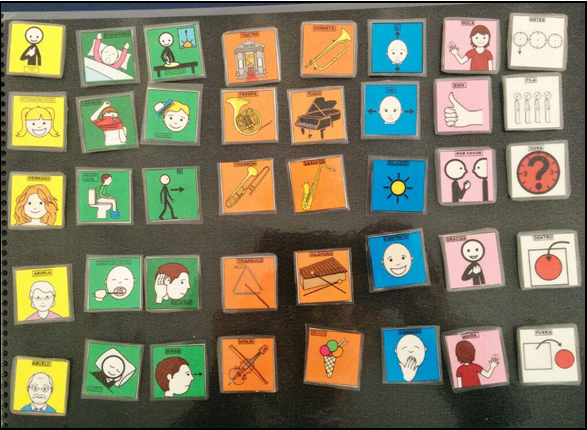
\includegraphics[width=0.7\linewidth]{Imagenes/Bitmap/tablerofisico}
	\caption{Pictographic board on which the user indicates what to communicate.}
	\label{fig:physicalboard}
\end{figure}


Communication boards are often created by teachers, parents or tutors to be used by a person with language difficulties. Traditionally they were made by cutting out and pasting pictograms on cardboard, but over time technological solutions have been implemented to facilitate this task. 

There are a multitude of applications that allow the creation of material based on pictograms, but they are generally limited to a specific format and offer little freedom to the user to create material. In addition, each of these applications has different options or facilities, such as translating a sentence into pictograms, a board where pictograms can be placed wherever you want, adding figures to the board, etc. But there is no single application that combines all these options. 
The purpose of this work is to create a web application that allows creating pictographic material quickly and easily, offering the greatest possible freedom to the user, and integrating the options most used and demanded by users in a single tool. 

\section{Objectives}
\label{cap1:sec:Objectives}



The aim of the work is to develop a web application that allows the creation of pictographic material by bringing together the functionalities most used and demanded by users. The application must have a board that allows to move with precision pictograms and other complementary elements.

For this purpose, the different existing applications will be investigated as well as the functionalities most demanded by users. Research will also be carried out into different web technologies.

Another objective is to create a simple and intuitive user interface that can be used in as many devices as possible. In order to verify the objectives of the work, an evaluation will be carried out to check the user-friendliness of the application. 


\section{Document structure}
\label{cap1:sec:mem}

The structure followed to organize this memory consists of the following chapters.
\begin{itemize}
	\item In chapter one, written in English and Spanish, it will set out the context in which the work has been carried out, also the motivation and objectives for doing so.
	
	\item Chapter two will explain briefly what a pictogram is and the different communication systems based on pictograms. In addition, the different tools related to pictograms will be discussed with an emphasis on editing communication boards.
	
	\item Chapter three will present the technologies used for the development of the application.
	
	\item Chapter four will specify the requirements and explain the created prototypes.
	
	\item Chapter five will detail the architecture and implementation of the application.
	
	\item Chapter six will show the design, results and analysis of the evaluation with users. 
	
	\item Chapter seven, written in English and Spanish, presents the final conclusions and specifies future work.
	
	\item Chapter eight will detail the tasks carried out by the two project participants.
\end{itemize}	




